\subsection{Títulos}
   \hypertarget{personal subsec:titulos}
   Se muestran en la figura \ref{fig:titulos_del_itba} los títulos y certificados relacionados a la carrera de grado.
   \begin{figure}
      \begin{center}
         \begin{subfigure}[b]{0.45\textwidth}
            
\includegraphics[width=\textwidth, frame]{titulo_itba.jpg}
            \caption{Título de Ingeniero Electrónico con especialidad en Telecomunicaciones del ITBA.}
            \label{fig:titulo_itba}
         \end{subfigure}%
         \hfill
         \begin{subfigure}[b]{0.45\textwidth}
            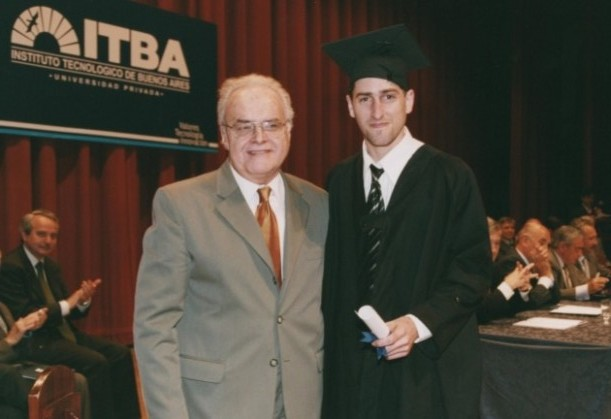
\includegraphics[width=\textwidth, frame]{foto_entrega_titulo.jpg}
            \caption{Foto de entrega de título junto con mi profesor y referente, el Ing. Eduardo Martinez.}
            \label{fig:foto_titulo}
         \end{subfigure} %
         \begin{subfigure}[b]{0.40\textwidth}
            \begin{center}
               
\includegraphics[width=0.6\textwidth, frame]{medalla_i+d_1.jpg}
               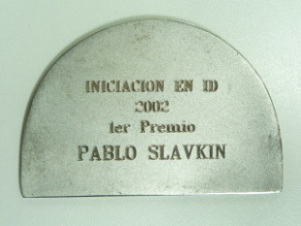
\includegraphics[width=0.6\textwidth, frame]{medalla_i+d_2.jpg}
               \caption{Medalla al primer puesto en I+D, iniciación en investigación y desarrollo, del ITBA}
               \label{fig:medalla_i+d}
            \end{center}
         \end{subfigure}%
         \hfill
         \begin{subfigure}[b]{0.55\textwidth}
            
\includegraphics[width=\textwidth, frame]{robot.jpg}
            \caption{Certificado de participación en Batletek, competencia de lucha de robots en el ITBA, en donde se obtuvo el tercer puesto.}
            \label{fig:foto_robot}
         \end{subfigure}%
      \caption{Títulos y certificados obtenidos durante la carrera de grado en el ITBA.}
      \label{fig:titulos_del_itba}
      \end{center}
   \end{figure}

   \begin{figure}
      \begin{center}
      \ContinuedFloat
         \begin{subfigure}[b]{0.40\textwidth}
            \begin{center}
               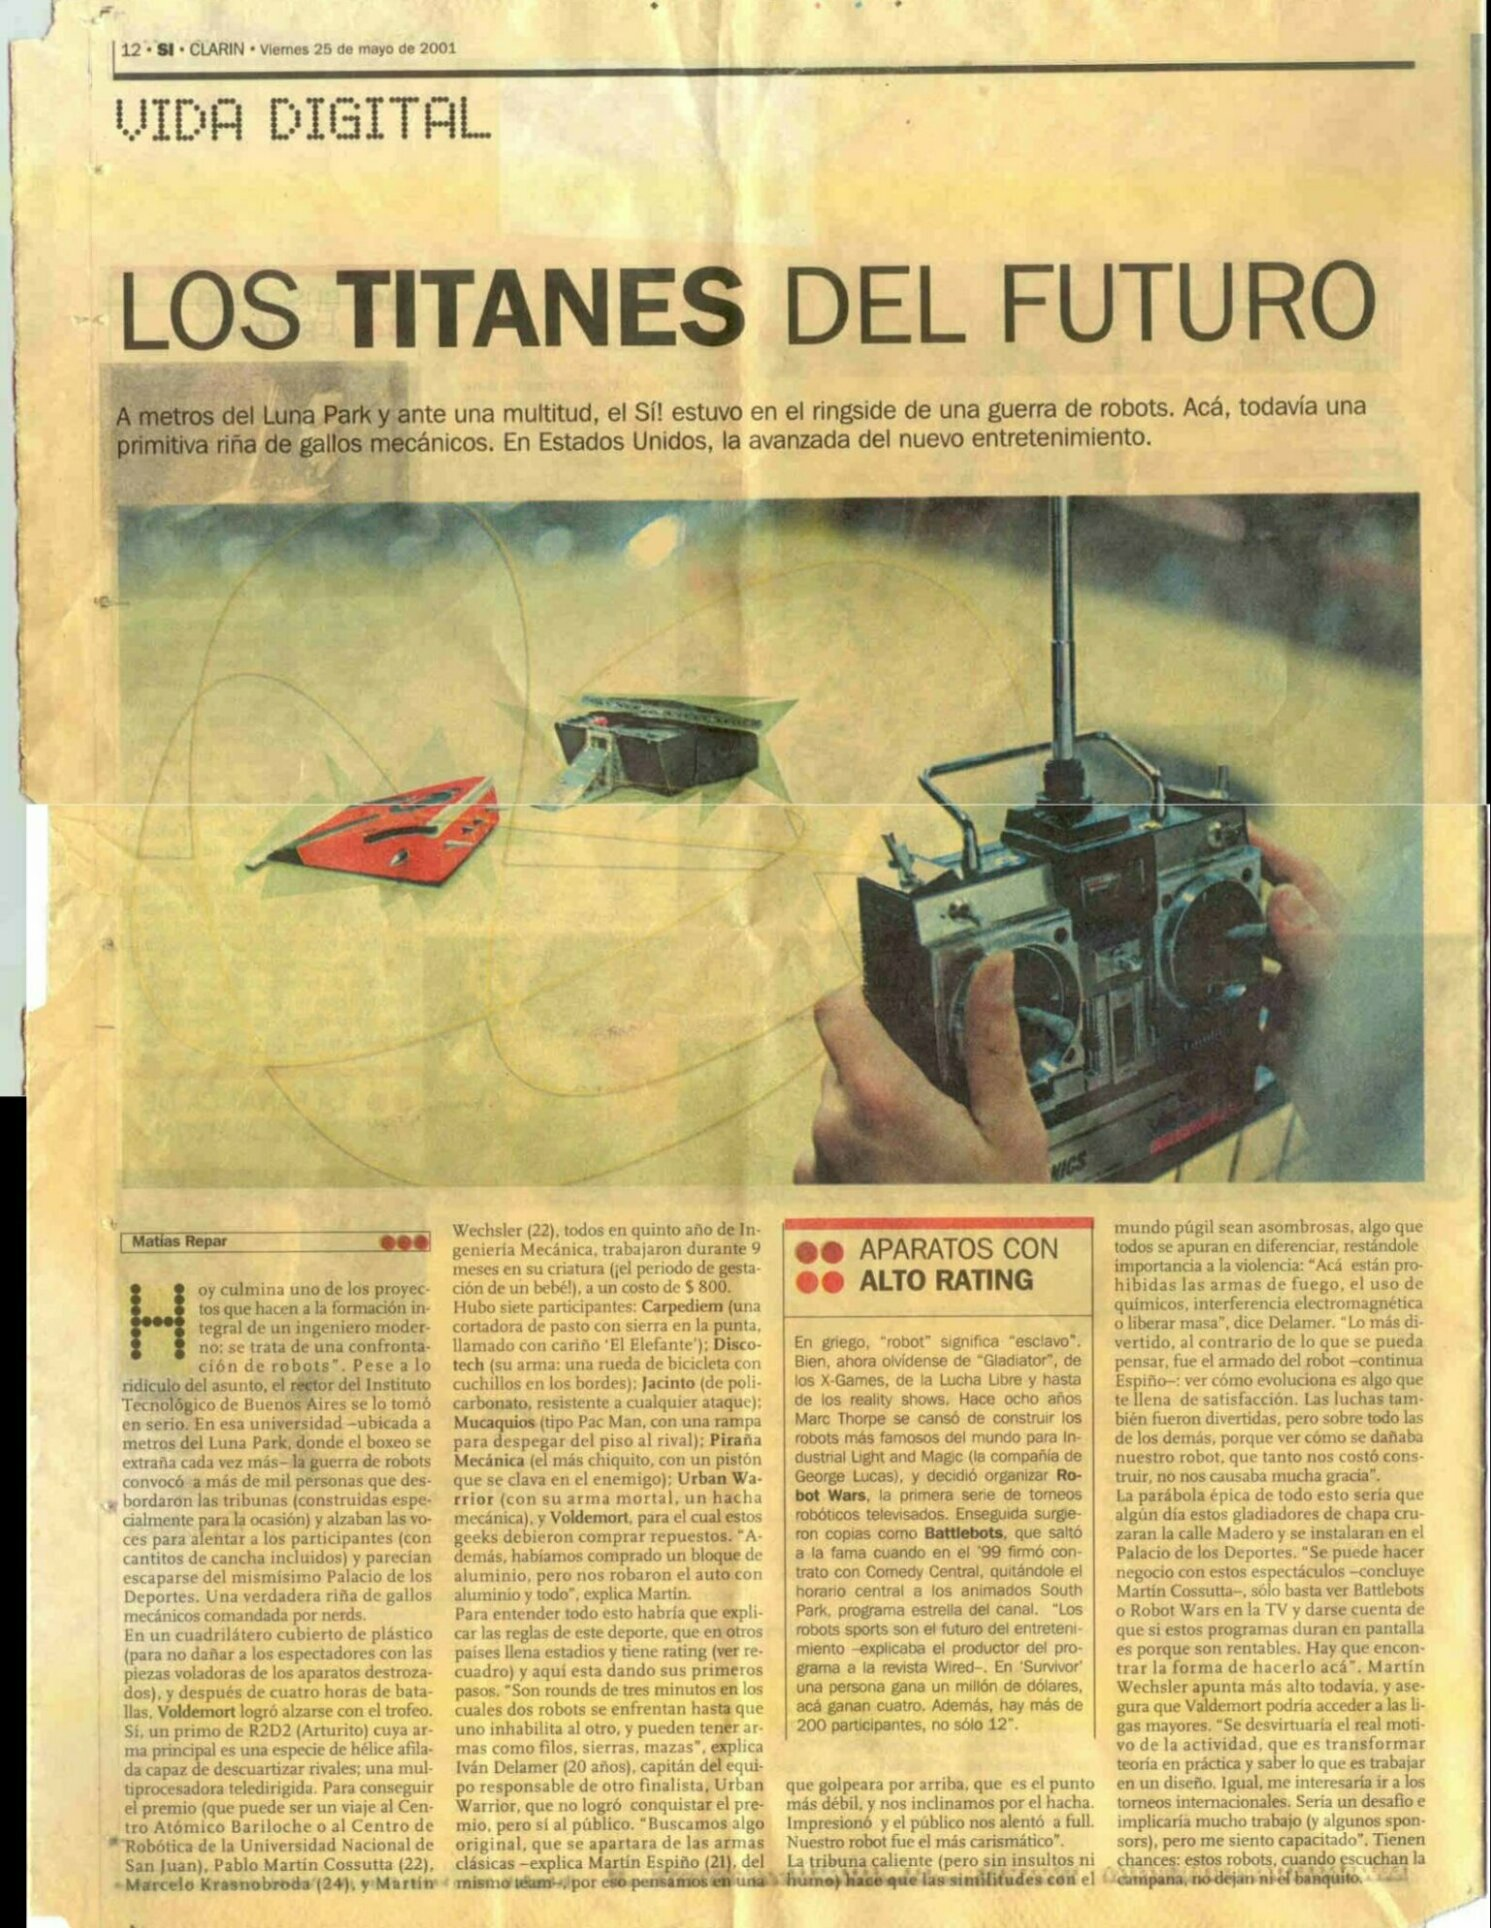
\includegraphics[width=\textwidth, frame]{robotdiario.jpg}
               \caption{Informe en diario Clarín sobre la competencia de robots de lucha en la que se participó.}
               \label{fig:robotdiario}
            \end{center}
         \end{subfigure}%
         \hfill
         \begin{subfigure}[b]{0.55\textwidth}
            
\includegraphics[width=\textwidth, frame]{inteligencia_artificial.jpg}
            \caption{Certificado de participación en el curso de Inteligencia Artificial.}
            \label{fig:foto_ai}
         \end{subfigure}%
      \caption{Títulos y certificados obtenidos durante la carrera de grado en el ITBA.}
      \label{fig:titulos_del_itba}
      \end{center}
   \end{figure}








   \begin{figure}
      \begin{center}
      \ContinuedFloat
         \begin{subfigure}[b]{0.45\textwidth}
            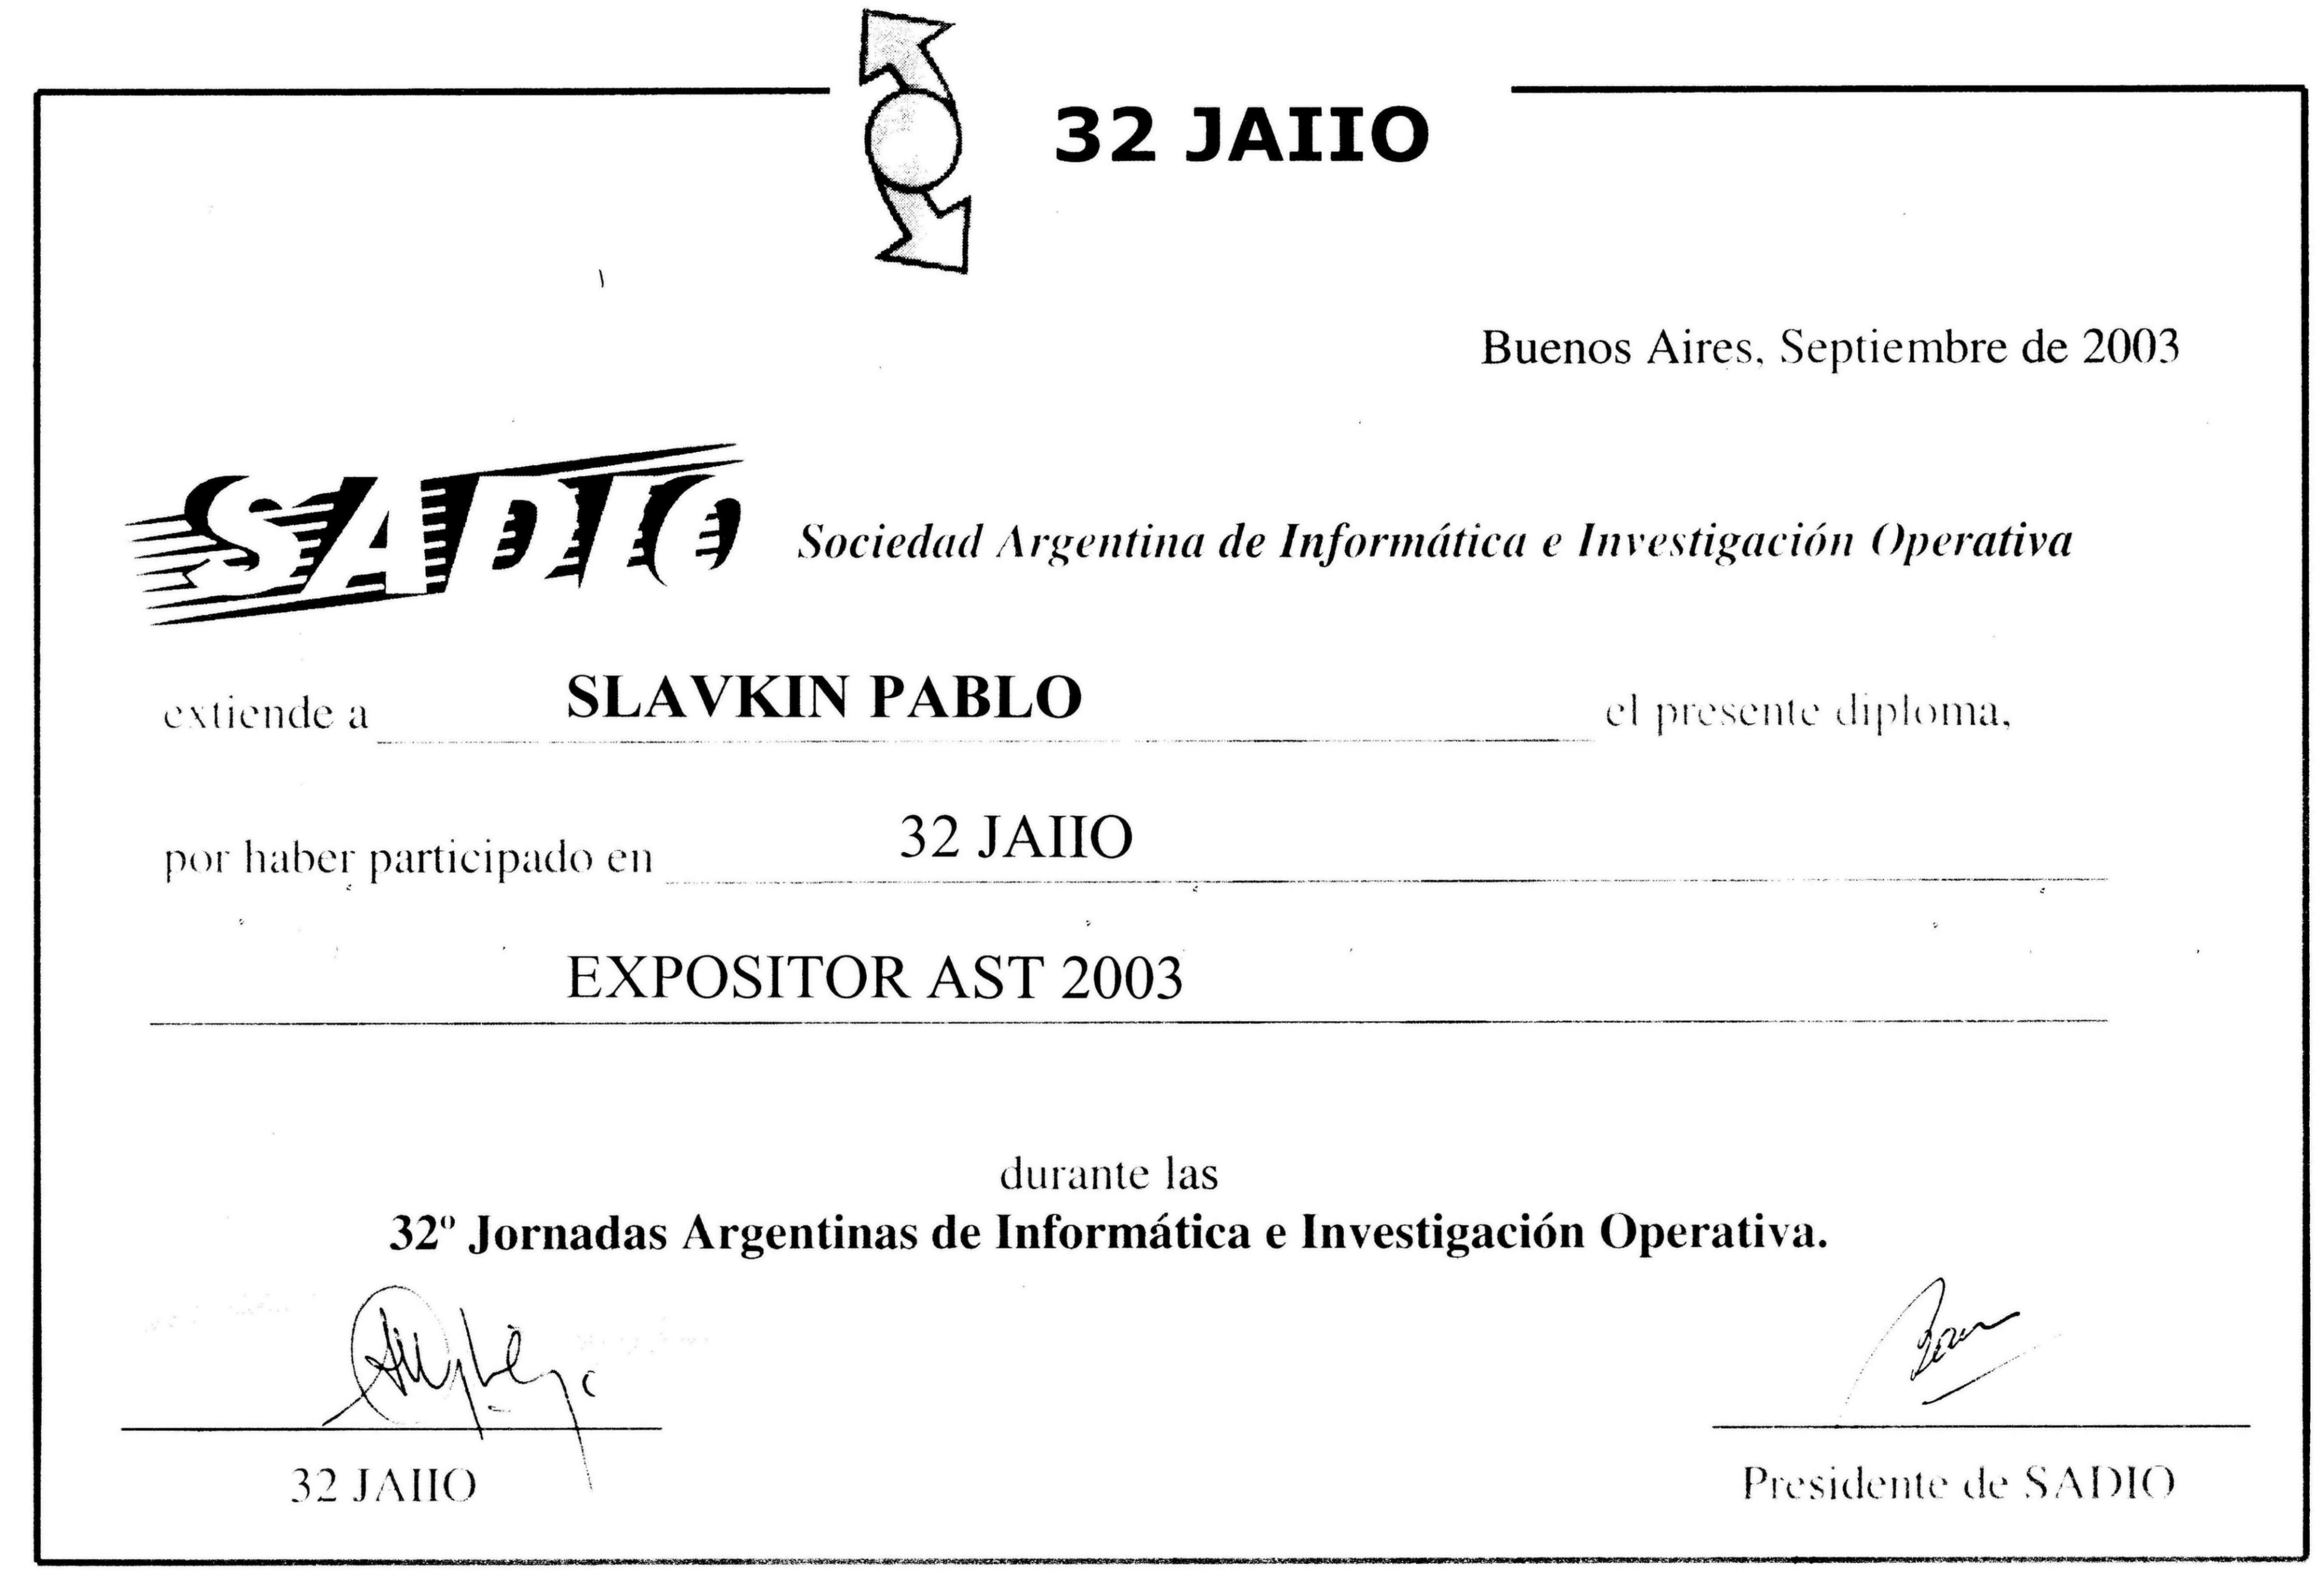
\includegraphics[width=\textwidth, frame]{sadio.jpg}
            \caption{JAIIO, 32\textsuperscript{o} Jornadas Argentinas de Informática e Investigación Aplicada. Se presento el trabajo \emph{Design and Simulation of a pipeline-structured Floating Point Unit for high performance general purpose processors.} \href{https://drive.google.com/open?id=15NkqA_rWbaObx1uiqe7ruBg9lWpIh5q7}{ver trabajo}}
            \label{fig:jaiio}
         \end{subfigure}%
         \hfill
         \begin{subfigure}[b]{0.45\textwidth}
            
\includegraphics[width=\textwidth, frame]{cacic.jpg}
            \caption{CACIC, IX Congreso Argentino de Ciencias de la Computación en donde se presento el trabajo \emph{Selection of the Optimum Stage Number in Pipelined Floating-Point Units} \href{https://drive.google.com/open?id=11z5qRrJ01Is6dx5NMHAOoXl3D0r2o8OY}{ver trabajo}}
            \label{fig:cacic}
         \end{subfigure}%
      \end{center}
      \caption{Títulos y certificados obtenidos durante la carrera de grado en el ITBA.}
      \label{fig:titulos_del_itba}
   \end{figure}




   En la figura \ref{fig:titulos_varios} se muestran certificados de diversas actividades realizadas de manera independiente.
   \begin{figure}
      \begin{center}
         \begin{subfigure}[b]{0.45\textwidth}
            
\includegraphics[width=\textwidth, frame]{courses/cursolatex.pdf}
            \caption{Introducción a {\LaTeX}. Se tomó el curso de introducción a {\LaTeX} como herramienta para la presentación de trabajos científicos y documentos en general. Se continuó luego de manera autodidacta y se la utiliza frecuentemente para la documentación, presentaciones, papers, etc. \href \linklatex {Ver certificado}}
            \label{fig:latex}
         \end{subfigure}%
         \hfill
         \begin{subfigure}[b]{0.45\textwidth}
            
\includegraphics[width=\textwidth, frame]{clase_robot_siglo21.jpg}
            \caption{Certificado por el dictado de un curso a escuela secundaria de introducción a la robótica, teórica y práctica. \href \linkrobotsiglo {Ver certificado}}
            \label{fig:robot_siglo_21}
         \end{subfigure}%

         \begin{subfigure}[b]{0.45\textwidth}
            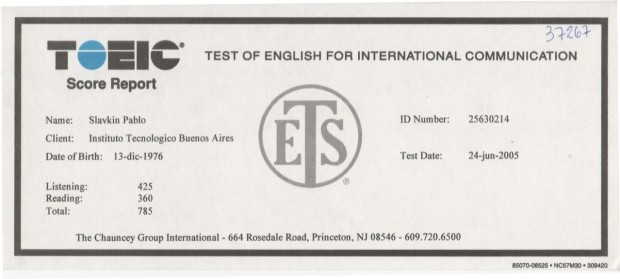
\includegraphics[width=\textwidth, frame]{courses/toeic.jpg}
            \caption{Certificado de examen de ingles TOEIC. \href \linktoeic {Ver certificado}}
            \label{fig:toeic}
         \end{subfigure}%
         \hfill
         \begin{subfigure}[b]{0.45\textwidth}
            
\includegraphics[width=\textwidth, frame]{courses/latam_2018.pdf}
            \caption{Diploma de participacion en el concurso de proyectos LATAM 2018 organizado entre el MIT y el ITBA. \href \linklatameigtheen {Ver certificado} }
            \label{fig:latam2018}
         \end{subfigure}%
         \hfill
         \begin{subfigure}[b]{0.45\textwidth}
            
\includegraphics[width=\textwidth, frame]{courses/latam_2020.pdf}
            \caption{Diploma de participacion en el concurso de proyectos LATAM 2020 organizado entre el MIT y el ITBA. \href \linklatamtwenty {Ver certificado} }
            \label{fig:latam2020}
         \end{subfigure}%
      \end{center}
      \caption{Certificados obtenidos en diferentes cursos y seminarios participando de manera independiente como parte de la actualización personal técnica y académica.}
      \label{fig:titulos_varios}
   \end{figure}


   En la figura \ref{fig:certificados_codility} se muestran certificados y premios obtenidos en la plataforma Codility que mide habilidades de programacion y codificacion en diferentes lenguajes.
   \begin{figure}
      \begin{center}
         \begin{subfigure}[b]{0.45\textwidth}
            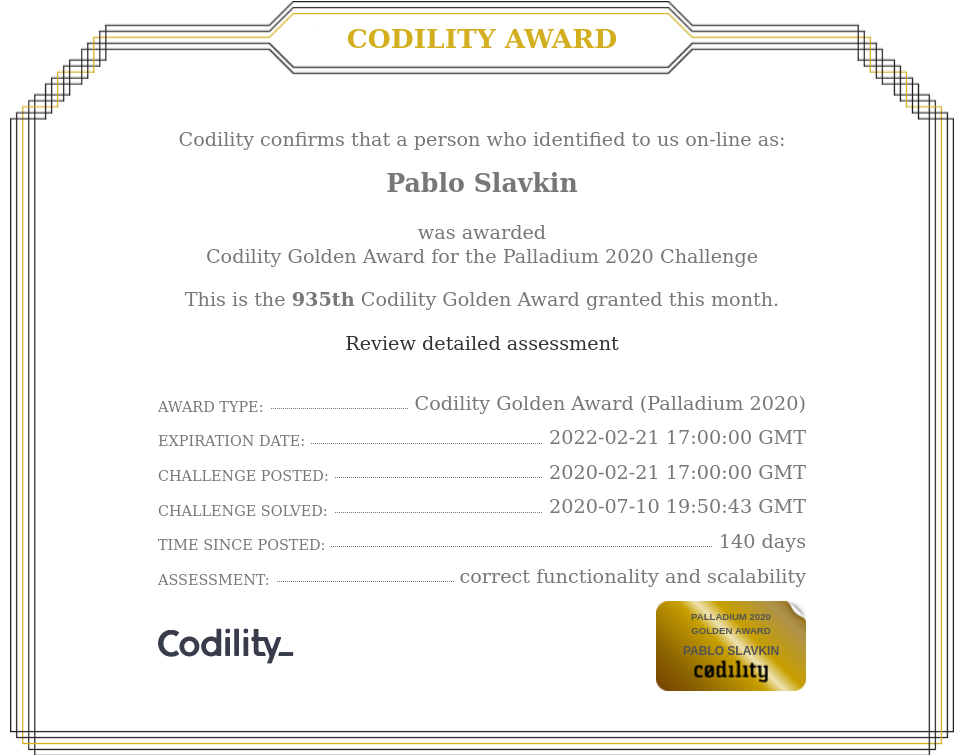
\includegraphics[width=\textwidth, frame]{codility_palladium_certificate.png}
            \caption{Premio de oro en el desafio Palladium 2020 de la plataforma Codility programado en C. \href {\linkcodilitycertone}{ver certificado}}
            \label{fig:latex}
         \end{subfigure}%
         \hfill
         \begin{subfigure}[b]{0.45\textwidth}
         \end{subfigure}%
      \end{center}

      \caption{Certificados obtenidos en la plataforma Codility.}
      \label{fig:certificados_codility}
   \end{figure}
